\section{Projekt}

In dem Projekt "`Home-Bacon"' wollen wir das Thema Lokalisation mittels Bluetooth-Beacons auf Smartwatches untersuchen und als Prototyp implementieren.

\subsection{Ergebnis}
Das Ergebnis unseres Projekts sind zwei mobile Applikationen, wobei die eine für ein Android-Smartphone und die andere für eine Android-Wear-Smartwatch entwickelt wird.

\subsection{Anwendungsfälle}
Wir möchten unsere Projektidee und unsere Anforderungen in Form von User-Storys und Anwendungsfällen konkretisieren. Dazu haben wir uns den fiktiven Anwender Anton ausgedacht, der sehr vergesslich aber experimentierfreudig ist. Als technikaffiner Mensch hat Anton natürlich eine moderne Smartwatch und ein Smartphone. Aufgrund seiner Vergesslichkeit wünscht sich Anton die Möglichkeit beim Verlassen eines Raumes an bestimmte Dinge erinnert zu werden. Beispielsweise möchte er beim Verlassen des Hauses an seine Einkaufsliste erinnert werden.

Nachfolgend werden Antons Wünsche detaillierter ausgeführt.

\subsubsection{Positionierung}
\begin{figure}[H]
\centering
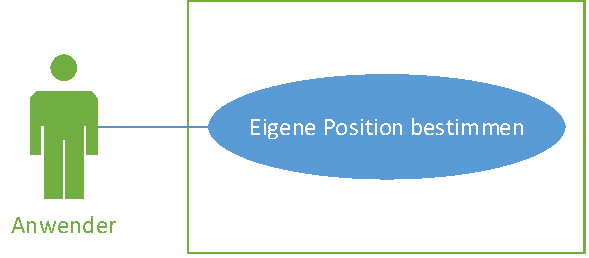
\includegraphics[width=0.7\linewidth]{Bilder/UseCase-Position}
\caption{Anwendungsfalldiagramm Positionierung}
\label{fig:UseCase-Position}
\end{figure}

\newpage
Als Anwender Anton möchte ich meine eigene Position in meinem Haus bestimmen können, um zu wissen in welchem Raum ich mich befindet. 

Akzeptanzkriterien:
\begin{itemize}
\item Die Smartwatch bestimmt die aktuelle Position.
\end{itemize}

Als Anwender Anton möchte ich wissen, wo sich ein verlegter Gegenstand befindet, um diesen leichter wiederfinden zu können.

Akzeptanzkriterien:
\begin{itemize}
\item Auf der Smartwatch kann aus allen getrackten Gegenstände der gesuchte ausgewählt werden.
\item Zu dem ausgewählten Gegenstand wird die zuletzt wahrgenommene Position angezeigt.
\item Die Smartwatch gibt Feedback abhängig von der Nähe zum Gegenstand.
\end{itemize}

\subsubsection{Notizen}
\begin{figure}[H]
\centering
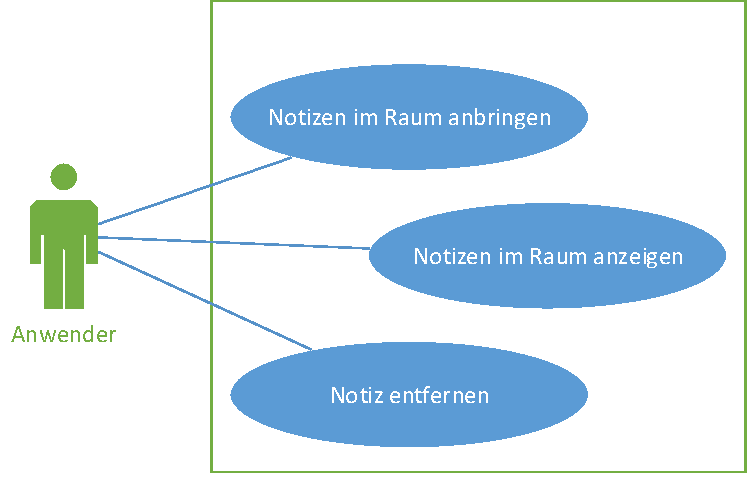
\includegraphics[width=0.7\linewidth]{Bilder/UseCase-Notizen}
\caption{Anwendungsfalldiagramm Notizen}
\label{fig:UseCase-Notizen}
\end{figure}

Als Anwender Anton möchte ich Notizen im Raum anbringen können, um diese zur späteren Ansicht zu hinterlassen.

Akzeptanzkriterien:
\begin{itemize}
\item Notizen können über das Smartphone im aktuellen Raum hinterlassen werden.
\end{itemize}

Als Anwender Anton möchte ich Notizen im Raum angezeigt bekommen, um hinterlassene Notizen zu lesen.

Akzeptanzkriterien:
\begin{itemize}
\item Auf der Smartwatch wird zuerst die aktuellste Notiz angezeigt.
\item Mithilfe der horizontalen Wischgeste sind ältere Notizen abrufbar.
\end{itemize}

Als Anwender Anton möchte ich Notizen löschen können, um alte Notizen zu entfernen.

Akzeptanzkriterien:
\begin{itemize}
\item Auf der Smartwatch kann mithilfe der vertikalen Wischgeste die angezeigte Notiz gelöscht werden.
\item Bevor die Notiz endgültig gelöscht wird, muss das Löschen bestätigt werden.
\end{itemize}

\subsubsection{Ereignisse}
\begin{figure}[H]
\centering
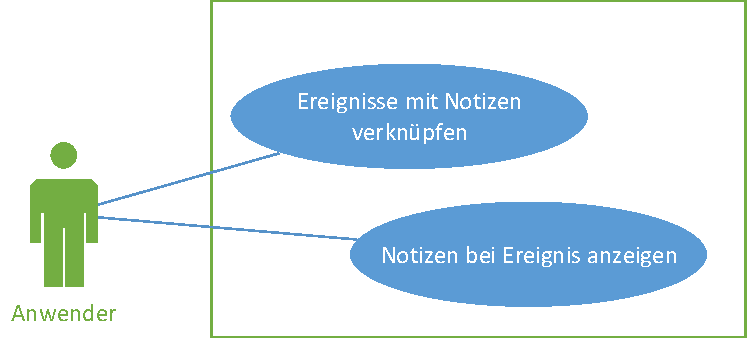
\includegraphics[width=0.7\linewidth]{Bilder/UseCase-Ereignisse}
\caption{Anwendungsfalldiagramm Ereignisse}
\label{fig:UseCase-Ereignisse}
\end{figure}

Als Anwender Anton möchte ich Ereignisse mit Notizen verknüpfen, um beim Verlassen bzw. Betreten eines Raumes die Notizen angezeigt zu bekommen.

Akzeptanzkriterien:
\begin{itemize}
\item Auf dem Smartphone können Notizen mit den zwei Ereignissen (Betreten bzw. Verlassen) verknüpft werden.
\end{itemize}

\newpage
Als Anwender Anton möchte ich die Notizen angezeigt bekommen, wenn ich einen Raum betrete bzw. verlasse, um an die Notiz erinnert zu werden.

Akzeptanzkriterien:
\begin{itemize}
\item Mittels der Smartwatch erhält Anton Feedback, wenn ein Ereignis mit verknüpften Notizen eintritt.
\item Auf der Smartwatch werden dann diese verknüpften Notizen angezeigt.
\end{itemize}


\subsection{Projektplan}

In folgendem Diagramm haben wir unsere Zeitplanung für das Projekt aufgezeichnet.

\begin{figure}[tbh]
\centering
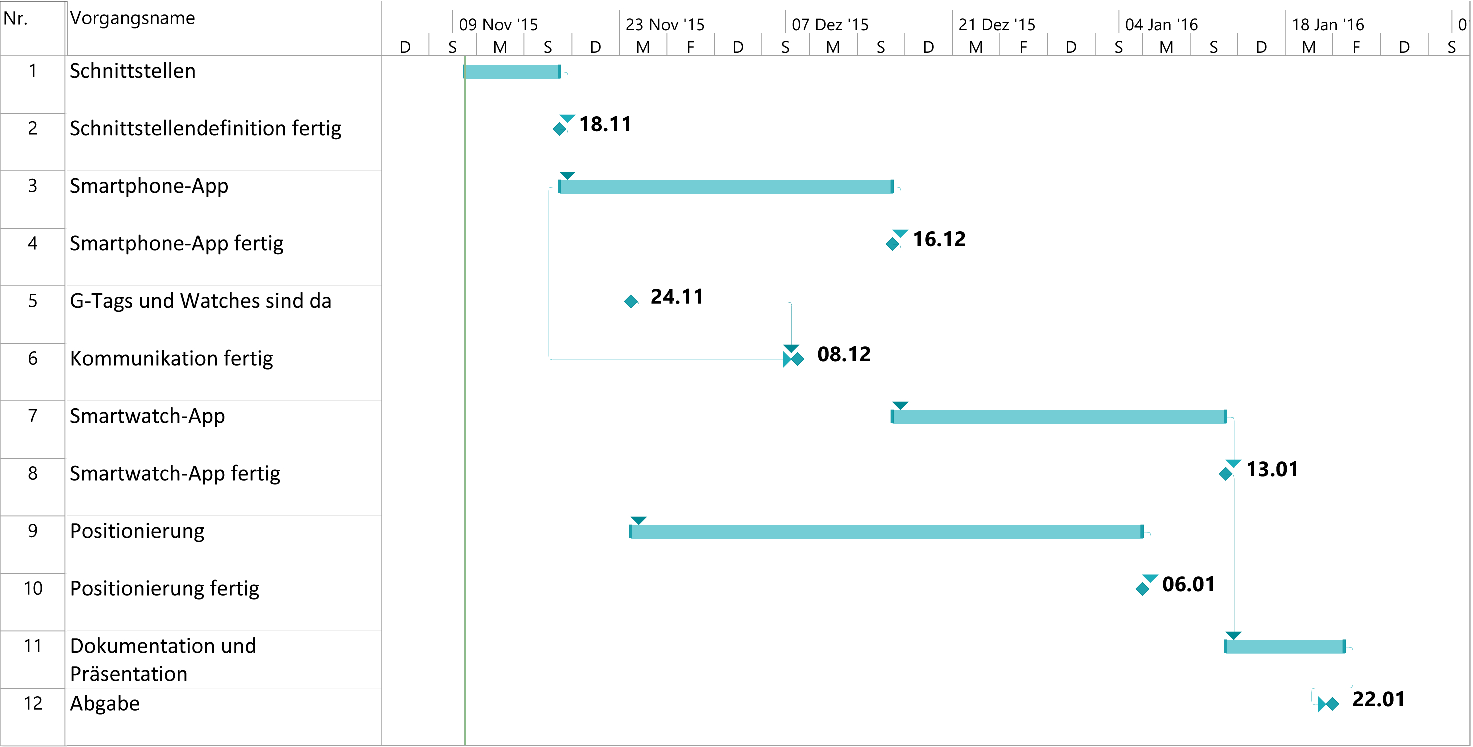
\includegraphics[width=1.0\linewidth]{Bilder/Projektplan}
\caption{Zeitplan mit Meilensteinen}
\label{fig:Zeitplan-1}
\end{figure}

\subsubsection{Projektphasen}
\begin{description}
	\item[Schnittstellen:] Definition der Schnittstellen zur Positionsbestimmung und zur Kommunikation zwischen
	Smartphone und Smartwatch. Dadurch können gewisse Teile unabhängig voneinander entwickelt werden.
	\item[Smartphone-App] Entwicklung der Smartphone-App zur Hinterlegung von Notizen in Räumen und bei Ereignissen.
	\item[Smartwatch-App] Entwicklung der Smartwatch-App zur Anzeige von Notizen in Räumen und bei Ereignissen sowie
	dem Wiederfinden von Gegenständen.
	\item[Positionierung] Bestimmung der Position der Smartwatch anhand der Bluetooth-Signale der stationären Tags.
	\item[Dokumentation und Präsentation] Erstellung der Dokumentation und Vorbereitung der Präsentation.
\end{description}

\subsubsection{Meilensteine}
\begin{description}
	\item[Schnittstellendefinition] Schnittstellen sind festegelegt.
	\item[G-Tags und Watches sind da] Geschätzter Termin für das Eintreffen der bestellten Ware.
	\item[Smartphone $\rightarrow$ Smartwatch] Kommunikation von der Smartphone-App mit der Smartwatch ist implementiert.
	\item[Smartphone-App] Die Smartphone-App ist fertig (ggf. Mock-Implementierungen für die Schnittstellen)
	\item[Positionierung] Die Positionierung auf der Smartwatch ist fertig.
	\item[Smartwatch-App] Die Smartwatch-App ist fertig.
	\item[Abgabe] Die Dokumentation wurde abgegeben.
\end{description}